\documentclass[12pt,journal,compsoc]{IEEEtran}
\usepackage{graphicx}
\newcommand\MYhyperrefoptions{bookmarks=true,bookmarksnumbered=true,
pdfpagemode={UseOutlines},plainpages=false,pdfpagelabels=true,
colorlinks=true,linkcolor={black},citecolor={black},pagecolor={black},
urlcolor={black},
pdftitle={Orbit Determination of 1951 Lick},
pdfsubject={Orbit Determination},
pdfauthor={Fengning Ding, Jason Liu, Patrick Rall},
pdfkeywords={Summer Science Program, 1951 Lick, Orbit Determination}}

\begin{document}

\title{Orbit Determination of 1951 Lick}

\author{Fengning~Ding,~Jason~Liu,~Patrick~Rall \\Summer Science Program Westmont 2011}%
\markboth{Orbit Determination of 1951 Lick}{}

\IEEEcompsoctitleabstractindextext{%
\begin{abstract}
\boldmath
Over the course of the Summer Science Program, the asteroid 1951 Lick was observed on seven days using a 14''~Meade telescope and the 24''~Keck Telescope at Westmont College.
From seventeen usable images, the right ascension and declination of the asteroid was measured using least-squares plate reductions.
By using Laplace's method of orbit determination and five iterations of differential corrections, we were able to compute the orbit of our asteroid.
Relative to an observation made on July 19, the ephemeris calculated from our orbital elements was within 0.112s for right ascension and 1.56'' declination of the observed coordinates of the asteroid determined using least-squares plate reductions.
The orbital elements from our analysis were consistent with previously determined measurements within statistical error.\end{abstract}
}

%and a 20.5 x 16.4 mm CCD Camera (1280 x 1024 pixels) 

\maketitle

\IEEEdisplaynotcompsoctitleabstractindextext
\IEEEpeerreviewmaketitle

\section{Introduction}
\IEEEPARstart{B}{ecause} 
of the potential of some near-earth asteroids to collide with the Earth, astronomers are especially interested in the orbits of near-earth asteroids.
To ensure accurate monitering of these hazardous objects moving in orbits perturbed by other planets, astronomers need to repeatedly measure the asteroid's position and velocity with high precision.
Furthermore, accurate orbital elements are needed for future astronomers to find the asteroid.

In July 2011, as part of the Summer Science Program at Westmont College, we determined the orbit of the asteroid 1951 Lick. We used a 14''~telescope and Westmont College's 24''~Keck Telescope to take seventeen images on seven different days to determine the asteroid's right ascension ($\alpha$) and declination ($\delta$) at a certain time. 
Another team performed similar measurements of 1951 Lick simultanously, and we shared data for Laplace's method of orbit determination.

Because the asteroid was leaving a retrograde loop, the equatorial unit vectors $\hat{\rho}$ from the Earth to the asteroid changed very slowly, causing the Gauss-Gibbs orbit determination method to fail.
However, by using Laplace's method and five iterations of differential corrections, we were able to determine the orbit of the asteroid and generate an ephemeris that accurately matches our observations.
Our orbit was described by the so-called "classical orbit elements": the semimajor axis $a$, the eccentricity $e$, the inclination (with respect to the plane of the Earth's orbit) $i$, the longitude of the ascending node (with respect to the Vernal Equinox) $\Omega$, the argument of the perihelion $\omega$, and the time of the last perihelion passage $T_p$.

\section{Methods}
To determine the orbital elements, images of the asteroid were taken using the two telescopes.
After median-combining these images into series to reduce noise, a least-squares plate reduction (LSPR) was performed using star coordinate data from the Naval Observatory Merged Astrometric Dataset (NOMAD) database. These reductions yielded $\alpha$ and $\delta$ for the asteroid at different times.
The orbital elements were determined using an implementation of Laplace's method of orbit determination with five iterations of differential corrections.

\subsection{Observing and Image Processing}
The asteroid was observed on seven days: July~1\footnote{As according to convention, all times are given in Universal Coordinated Time (UTC) unless otherwise specified.}, July~3, July~8, July~10, July~16, July~19, and July~25 at around 4:00-6:00 UTC each day.
First, the approximate apparent $\alpha$ and $\delta$ of the asteroid was researched using NASA's Jet Propulsion Laboratory's HORIZONS ephemeris computation service (JPL HORIZONS).
Software Bisque's TheSkyX software was used to generate a starchart of the region of the sky in which the asteroid would be located.
After syncing and focusing the telescope on a nearby star, three or four series of five or seven images were taken with an exposure time of 45 seconds per image. For details see Table~\ref{tab:serieslist}. 

When retrieving the approximate $\alpha$ and $\delta$ from JPL HORIZONS, data was collected for the apparent $\alpha$ and $\delta$, which compensates for various systematic errors such as atmospheric distortion.
However, our telescopes already made these corrections, and so the asteroid was always located significanly off the center of the image.
This error was only discovered and corrected after July 19. 

To remove noise and several `hot pixels' (pixels that had been overexposed by a cosmic ray), the images for each series were flat-field corrected, manually aligned, and median combined using Diffraction Limited's MaxIm DL software.
The location of the asteroid was seen on the images by `blinking' (changing images over a short time period) aligned versions of the combined series.
For an example of a processed image see Fig.~\ref{fig:exampleseries}.

\begin{figure}[!t]
\centering
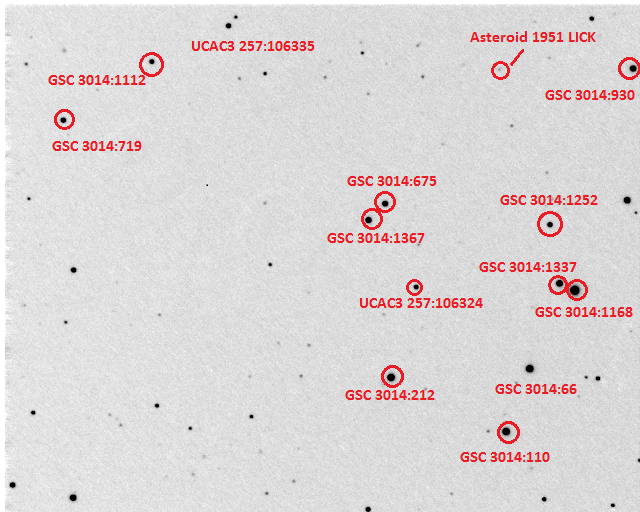
\includegraphics[width=3.4in]{Jul10Series2.png}
\caption{An example of a combined series of images: Series 2 of the observation on July 10 using the Meade 14'' Telescope.\label{fig:exampleseries}}
\label{fig_sim}
\end{figure}

\begin{table}[!t]
\centering
\begin{tabular}{|c|c|c|c|c|}
\hline
Date & Telescope & Sync Star & Filter & \# images \\ \hline \hline
July 1 &Meade 14''& \multicolumn{3}{c|}{Ommited due to bad quality}\\ \hline \hline
July 3 & DFM 24''& Arcturis  & Clear & 5 \\ \cline{4-5}
 & & & Clear & 5\\ \cline{3-5}
 & & \multicolumn{3}{c|}{Ommited due to bad quality} \\ \hline \hline
July 8 &  Meade 14''  &\multicolumn{3}{c|}{Images are of wrong part of sky} \\ \cline{3-5}
 & & Pheceta & Clear & 7 \\ \cline{4-5}
 & & & Clear & 7\\ \cline{4-5}
 & & & Clear & 7\\ \hline \hline
July 10 & Meade 14''& Pheceta  & Clear &7 \\ \cline{4-5}
 & & & Clear & 7\\ \cline{4-5}
 & & & Clear & 7\\ \hline \hline
July 16 & Meade 14''& Pheceta  & V-filter &5 \\ \cline{4-5}
 & & & Clear & 5\\ \cline{4-5}
 & & & Clear & 5\\ \cline{4-5}
 & & & Clear & 5\\ \cline{4-5}
 & & & Clear & 5\\ \hline \hline
July 19 & Meade 14''& Pheceta  & Clear &7 \\ \cline{4-5}
 & & & Clear & 7\\ \cline{4-5}
 & & & Clear & 7\\ \cline{4-5}
 & & & Clear & 7\\ \hline \hline
July 25 & Meade 14'' & Pheceta  & Clear &5 \\ \cline{4-5}
 & & & V-filter & 1\\ \hline 
\end{tabular}
\caption{List of series taken in observations \label{tab:serieslist}}
\end{table}

\subsection{Least-Squares Plate Reduction}
Using a Python program, LSPR was performed on each series of images.
The centroids of numerous bright reference stars were obtained using MaxIm DL and compiled in a document along with the stars' $\alpha$ and $\delta$ as given by NOMAD. 

To find the coordinates of the asteroid a planar fit was applied to the images, followed by a procedure to correct for the spherical shape of the sky.
Failure to compensate for the spherical shape of the sky causes the equatorial coordinates obtained from the first least squares fit to be off near the edges of the image.
First, by using the time of observation given by the FITS header of each image (and taking into account the difference between our observatory's clock and the US Naval Observatory's clock), the local sidereal time was calculated to convert the equatorial coordinates of each reference star into the local coordinates of altitude and azimuth.
Assuming an index of refraction of $n-1=58.2''$ for the atmosphere, the computed altitude of each star was adjusted to account for the refraction of light by the atmosphere.
The adjusted altitude and azimuth were then converted back to equatorial coordinates.

Then, assuming that the image covers a flat portion of the sky, the program first computes a least-squares linear fit that maps the $x$,$y$-plate coordinates of each star to its apparent equatorial coordinates.
Using this mapping, the equatorial coordinates of the center of the image were obtained to calculate the standard $\xi$,$\eta$-coordinates for each reference star\footnote{See [2]}. Because the standard coordinates are linear with respect to the plate coordinates, a more accurate least-squares fit was computed that maps the plate coordinates to the standard coordinates. 
Using this linear transformation, the $\xi$,$\eta$-coordinates of the asteroid was obtained, from which the apparent $\alpha$,$\delta$ of the asteroid was calculated.
Finally, the apparent equatorial coordinates was transformed back into equatorial coordinates using the same index of refraction of the atmosphere.

To obtain an estimate of the uncertainty of the $\alpha$, $\delta$ of the asteroid, the deviation of the predicted equatorial coordinates of each star and the catalogued coordinates was computed with two degrees of freedom.
This residual was due to defects in the CCD chip and telescope mirror, abberation of starlight, inaccurate tabulations of reference star coordinates, and uncertainties in the centroid computations.

\subsection{Orbit Determination using Laplace's Method}
From the measured $\alpha$ and $\delta$ of the asteroid, the classical orbital elements of the asteroid was determined. Because the equatorial coordinates of the asteroid changed very little
%Pato: personally, I would like these to be quantified. How much is very little? Why exactly is this a problem for convergence of Gauss-Gibbs?
over the course of our observations, the Gauss-Gibbs method of orbit determination\footnote{Described in [1]} produced unrealistic results, and so Laplace's method was used. 

We used five observations to obtain $\frac{d\hat{\rho}}{d\tau}$ and $\frac{d^2\hat{\rho}}{d\tau^2}$ for the middle observation\footnote{$\tau$ is the modified time given by $\tau=kt$, for ordinary time $t$ and the Gaussian gravitation constant $k=0.017...$.
All time derivatives in this section are with respect to modified time}. 
The five unit equatorial vector are labeled $\hat{\rho}_1$, $\hat{\rho}_2$, $\hat{\rho}_3$, $\hat{\rho}_4$, $\hat{\rho}_5$. The middle three observations were made on July 8 and are used to calculate $\frac{d\hat{\rho}}{d\tau}$.
The second derivative of $\hat{\rho}$ at the middle observation was  computed using  $\hat{\rho}_1$, $\hat{\rho}_3$, and  $\hat{\rho}_5$, which were made on June 27, July 8, and July 25 respectively\footnote{The June 27 data was obtained by the other team}.
This time span was chosen to be large enough for the first derivative to change appreciably.

To compute the first derivative, we used the second-order Taylor expansion:
\begin{eqnarray*}
\hat{\rho}_4&=&\hat{\rho}_3+\hat{\rho}_3' (\tau_4-\tau_3)+\frac{1}{2}\hat{\rho}_3'' (\tau_4-\tau_3)^2\\
\hat{\rho}_2&=&\hat{\rho}_3+\hat{\rho}_3' (\tau_2-\tau_3)+\frac{1}{2}\hat{\rho}_3'' (\tau_2-\tau_3) ^2\\
\end{eqnarray*}
from which we solved for $\hat{\rho_3}'$.
The second derivative was calculated similarly but with   $\hat{\rho}_1$ and $\hat{\rho}_5$ instead.
From $\frac{d\hat{\rho}}{d\tau}$ and $\frac{d^2\hat{\rho}}{d\tau^2}$, the standard Laplace method was used to generate the position and velocity vectors of the asteroid\footnote{See [1]}.
This calculation was done using a Python program.

From the preliminary position and velocity, an ephemeris was generated for the times of each of our observations, and the differences from the measured values, $\Delta \alpha$ and $\Delta \delta$, was calculated.
A small change in the position and velocity changes $\alpha$ and $\delta$ according to the equations below:
\begin{eqnarray*}
\Delta \alpha &=& \frac{\partial \alpha}{\partial r_x} \Delta r_x + \frac{\partial \alpha}{\partial r_y} \Delta r_y + \frac{\partial \alpha}{\partial r_z} \Delta r_z + \\& &
\frac{\partial \alpha}{\partial v_x} \Delta v_x + \frac{\partial \alpha}{\partial v_y} \Delta v_y + \frac{\partial \alpha}{\partial v_z} \Delta v_z   \\
\Delta \delta &=& \frac{\partial \delta}{\partial r_x} \Delta r_x + \frac{\partial \delta}{\partial r_y} \Delta r_y + \frac{\partial \delta}{\partial r_z} \Delta r_z + \\& &
\frac{\partial \delta}{\partial v_x} \Delta v_x + \frac{\partial \delta}{\partial v_y} \Delta v_y + \frac{\partial \delta}{\partial v_z} \Delta v_z
\end{eqnarray*}
Using six observations of our asteroid, we found least-squares corrections $\Delta r_x$, $\Delta r_y$, $\Delta r_z$, $\Delta v_x$, $\Delta v_y$, and $\Delta v_z$ for the position and velocity vectors.
Due to inaccurate preliminary position and velocities, these corrected position and velocity vectors were still not accurate (since the differential corrections described above only correct for small inaccuracies), and so the corrected position and velocity vectors were corrected again.
This process was iterated five times until the computed orbital elements converged.

To compute the uncertainties for the orbital elements, we assumed that the $\alpha$ and $\delta$ of the asteroid was distributed normally according to the standard deviation computed from the LSPR.
A Monte-Carlo method with sample size of five hundred was used to compute the orbital elements using the procedure specified above for a set of asteroid coordinates randomly sampled from the Gaussian distribution.
The standard deviation of the computed orbital elements was reported as the uncertainty.

\subsection{Photometry}
On July 16 and July 25, a V-filter image of the asteroid was taken to measure the V-magnitude of the asteroid.
To determine the apparent magnitude of the asteroid, images were first taken with a Green V-Filter in the telescope, instead of the clear filter that is customarily used.
This V-Filter allows accurate measurements of magnitudes of stars.
After taking a series of images with the V-Filter, V-Magnitudes of surrounding stars were researched in TheSkyX.
The V-Filter images were calibrated in MaxIm DL by setting the magnitude of the reference stars equal to the V-Mag from TheSkyX.
Afterwards, the asteroid was selected, and the V-Mag of the asteroid was able to be read. 

\begin{table}[!t]
\centering
\scalebox{0.9}{
\begin{tabular}{|c|c|c|}
\hline
Asteroid V-Mag & Observation & Sync Star VMag \\ \hline \hline
16.861 &  GSC 2531:1730 & 12.690 \\ \hline
17.122 &  GSC 2529:1728 & 12.590 \\ \hline
\end{tabular}
}
\caption{V-Magnitude of 1951 Lick \label{tab:vmag}}
\end{table}

\section{Results}

The result of the orbit determation along with the uncertainty are shown in Table~\ref{tab:orbitalelements}.

\begin{table}[!t]
\centering
\scalebox{0.9}{
\begin{tabular}{|c|c|c|}
\hline
$a$ & $e$ & $i$ \\ \hline
$1.3894 \pm 0.0094$ AU & $0.06053  \pm 0.0024$ & $39.089 \pm 0.019 ^{\circ}$  \\ \hline \hline
$\Omega$ & $\omega$ & $T_P$ \\ \hline
$130.7706 \pm 0.1415 ^{\circ}$  & $140.65 \pm 3.71 ^{\circ}$ & $2455237.7 \pm 11.3$ JD \\ \hline
\end{tabular}
}
\caption{Measured orbital elements \label{tab:orbitalelements}}
\end{table}

We note that the orbit of the asteroid is similar in eccentricity to that of Mars (with $e = 0.093$\cite{bib:horizons}) and the point of perihelion is hard to distinguish from other points, so the values for $\omega$ and $T_p$ are harder to determine. 

\begin{figure}[!t]
\centering
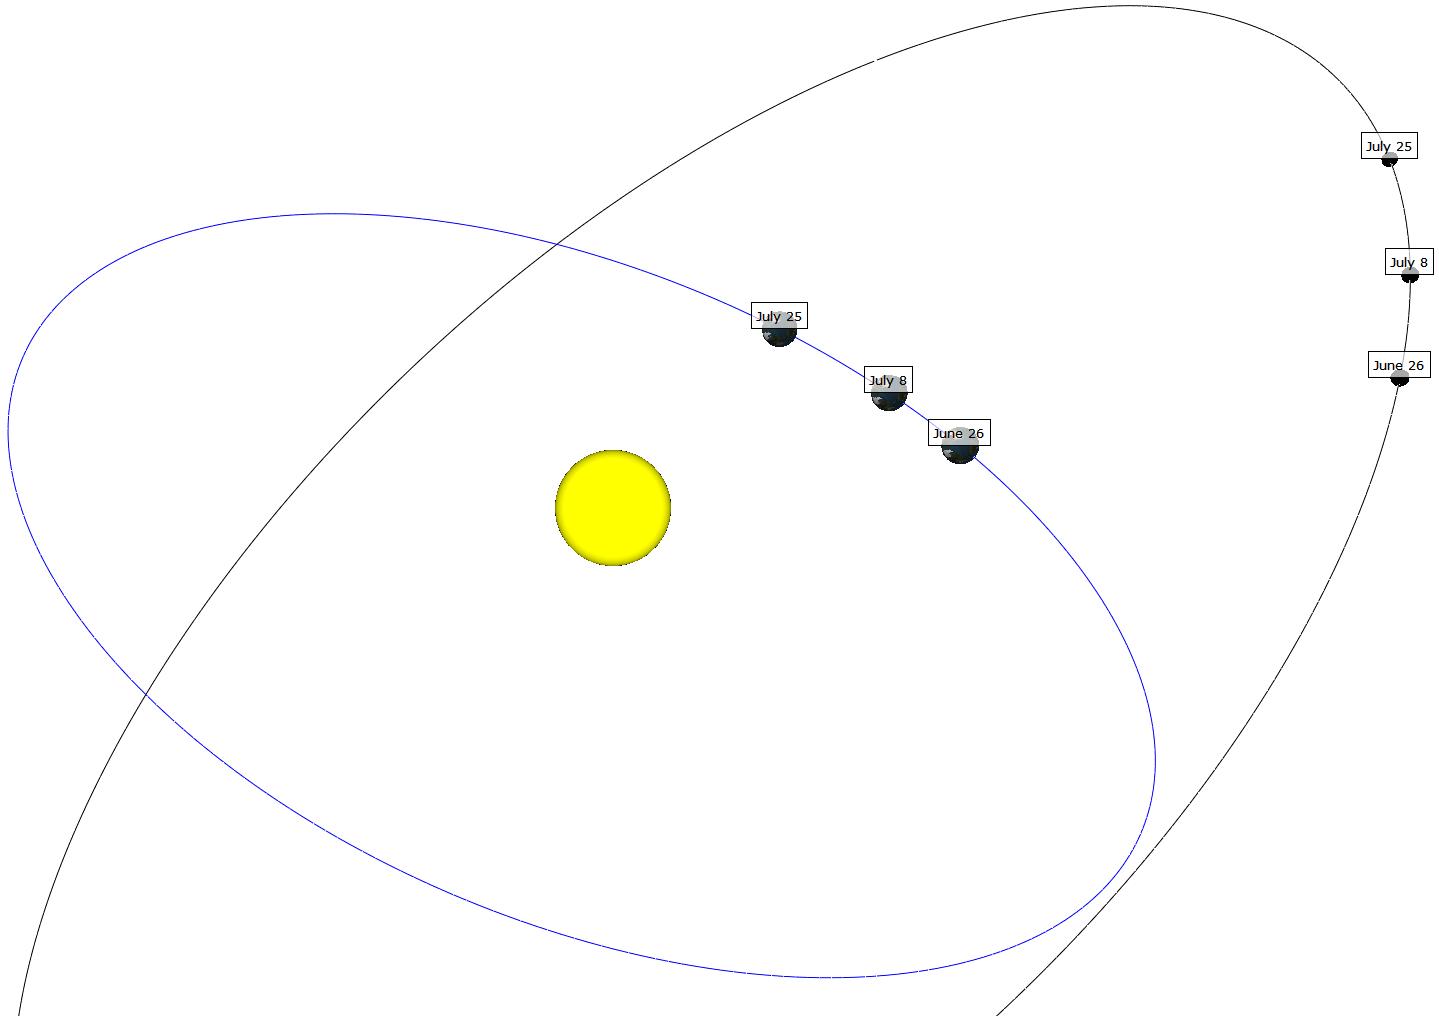
\includegraphics[width=3.5in]{LICK_Orbit2.png}
\caption{Position of the asteroid relative to the Earth}
\label{fig_sim}
\end{figure}

\section{Conclusion}
JPL HORIZONS provides values for the orbital elements, which serve as a good comparison to our data.
The differences between the orbital elements that were determined in the experimental procedure and those given by JPL are shown in Table~\ref{tab:HORIZONScomparison}.
The difference between the values is always significantly less than the statistical errors - there are no discrepancies.
To compare the accuracy of the two orbital elements, the ephemerides produced by the datasets can be compared to our observations, as seen in Table~\ref{tab:observationcomparison}.
It is clear that the measured orbital elements produce a closer value than that of HORIZONS.
Thus, the determined orbital elements constitute an improvement on the currently accepted values.

\begin{table}[!t]
\centering
\scalebox{0.9}{
\begin{tabular}{|c|c|c|c|}
\hline
Quantity & Measurement & HORIZONS Value & Difference \\ \hline
$a$ & $1.3894 \pm 0.0094$ AU & 1.390536 AU & 0.0011 AU \\ \hline
$e$ & $0.06053  \pm 0.0024$  & 0.0616082 & 0.0011 \\ \hline
$i$ & $39.089 \pm 0.019^{\circ}$ & 39.08962$^{\circ}$ & 0.001$^{\circ}$\\ \hline
$\Omega$ & $130.7706 \pm 0.1415 ^{\circ}$ & 130.769445$^{\circ}$ & 0.0012$^{\circ}$\\ \hline
$\omega$ & $140.65 \pm 3.71 ^{\circ}$ &140.4418$^{\circ}$ & 0.21$^{\circ}$\\ \hline
$T_P$ & $2455237.7 \pm 11.3$ JD & 2455835.571 JD & 2.1 JD \\ \hline
\end{tabular}
}
\caption{Measured orbital elements in comparison with JPL HORIZONS orbital elements \label{tab:HORIZONScomparison}}
\end{table}

\begin{table}[!t]
\centering
\scalebox{0.9}{
\begin{tabular}{|c|c|c|c|}
\hline
Date & Observed $\alpha$ & HORIZONS $\alpha$ & Computed $\alpha$ \\
\cline{2-4} & Observed $\delta$ & HORIZONS $\delta$  & Computed $\delta$ \\ \hline \hline
Jul 19 & 12h 24m 7.855s &  12h 24m 3.18s & 12h 24m 7.667s \\
\cline{2-4} & 35$^{\circ}$ 5' 27.33'' & 35$^{\circ}$ 5' 32.0'' &  35$^{\circ}$ 5' 28.89'' \\ \hline
\end{tabular}
}
\caption{Comparison of JPL HORIZONS ephemeredes and ephemeredes from determined orbital elements with observation data\label{tab:observationcomparison}}
\end{table}

From the orbital elements, it is clear that there is very low probability the asteroid will hit the Earth in the near future.
With such a low eccentricity, the asteroid is in a highly circular orbit, minimizing perturbations from other planets.
Since gravitational acceleration is independent of mass, the stability of the asteroid's orbit is comparable to that of Mars in the short term.

The successful computation of the orbit of 1951 Lick is an interesting case study, considering the non-ideal location of our asteroid with respect to the Earth.
Future groups would benefit from our method of orbit determination.

\section*{Acknowledgments}

The authors would like to thank Dr. Michael Faison, Mr. Martin Mason, and Mary Masterman, Dougal Sutherland, Becky Raph, and Sean Mattingly for their help debugging our Python programs, observations, and teaching us the methodology used in this project.

\begin{thebibliography}{1}
\bibitem{bib:Danby}
J.M.A. ~Danby \emph{Fundamentals of Celestial Mechanics}, 1st~ed.\hskip 1em plus
  0.5em minus 0.4em\relax New York: Macmillan, 1962.
\bibitem{bib:Tatum}
J.B~Tatum \emph{Celestial Mechanics}, 1st~ed., 2002\hskip 1em plus
  0.5em minus 0.4em\relax Obtained from M. Mason in 2011
\bibitem{bib:horizons}
    JPL Horizons
%Cite me properly
\end{thebibliography}

\end{document}